Il sistema operativo \`e un programma che controlla l'esecuzione dei ``programmi applicativi''. Un'interfaccia fra applicazioni ed hardware.

Un sistema operativo \`e caratterizzato dall'insieme delle chiamate di sistema (system call). Il sistema operativo ``esporta'' al programmatore un insieme di ``procedure'', un'interfaccia di programmazione unica ad ogni sistema operativo.

Il software del sistema operativo \`e un manager dell'hardware (o delle risorse). Non si pu\`o andare \textit{sotto} il sistema operativo, non si pu\`o accedere direttamente alle risorse hardware.

Una system call primitiva pu\`o essere l'open di un file.

I/O controller = interfaccia software o ``digitale'' fra sistema operativo e dispositivo I/O.

I/O device = il dispositivo fisico o analogico di I/O.

I sistemi operativi moderni sono molto grandi, e non tutto pu\`o essere tenuto in ram. La parte che resta in ram \`e chiamata storicamente \textit{kernel}. Contiene le funzioni pi\`u utilizzate. La funzione pi\`u usata \`e quella che si occupa di assegnare un programma al processore. I sistemi operativi ``micro-kernel'' hanno \textit{solo} questo programma.

I SO inizialmente venivano chiamati ``batch system''. Prendevano una funzione alla volta e la eseguivano. I programmi, caricati uno alla volta in ram, dovevano contenere alla fine un'istruzione (di salto) per restituire il controllo al sistema operativo. Questo approccio \`e chiamato ``uniprogrammazione''

La percentuale di utilizzo della CPU con un batch system si calcola dividendo il numero di microsecondi in cui il programma esegue istruzioni per il numero di microsecondi che il programma impiega in totale per eseguire il programma.

Ad esempio, un programma che impiega 30 microsecondi in lettura e scrittura ed un microsecondo in elaborazione, usa il $3,2\%$ della CPU.

L'idea di multiprogrammazione \`e di eseguire pi\`u programmi contemporaneamente. Quando un programma \`e in I/O, il processore esegue un altro programma.

Ammettendo di avere una situazione simile alla precedente, 30 microsecondi di I/O e 1 microsecondo di elaborazione, ma tre programmi in esecuzione contemporaneamente. Il tempo totale \`e di 33 microsecondi. Dividendo i 3 microsecondi di elaborazione per i 33 di impiego totale, l'utilizzo della CPU diventa del $9\%$, triplicato rispetto al sistema uniprogrammato in cui i tre processi sarebbero stati eseguiti uno dopo l'altro.

Un programma interattivo \`e un programma che interagisce con il terminale. Un programma interattivo solitamente usa pochissima CPU, ma molta memoria.

I sistemi time sharing sono pensati per l'interazione con le persone. Ogni programma ha una ``finestra'' di tempo fissata disponibile per l'accesso al processore, dopo la quale finisce in fondo alla coda ed il programma successivo viene messo in esecuzione.

Il sistema operativo introduce delle astrazioni che facilitano il lavoro. Una di queste \`e l'astrazione del ``processo''.

\begin{itemize}
    \item Un processo \`e un programma in esecuzione. \`E un qualcosa di dinamico. In ogni istante, il programma in esecuzione ha modificato certe risorse del sistema: dati sul disco, dati in memoria. In ogni istante \`e caratterizzato quindi da uno stato, quello delle risorse a cui accede.
    \item Un processo \`e un'attivit\`a caratterizzata dall'esecuzione di una sequenza di istruzioni, \`e associato ad uno stato corrente (l'insieme di dati e risorse che il processo ha modificato), e un insieme di istruzioni di sistema.
    \item Un processo \`e l'istanza di un programma in esecuzione su un computer.
    \item Un processo \`e quell'entit\`a che pu\`o essere assegnata ed eseguita su un processore. Non \`e la singola istruzione, ma tutto l'ambiente in cui quell'istruzione deve essere eseguita: variabili in memoria, risorse, file da utilizzare.
\end{itemize}

Elementi caratterizzanti di un processo in un qualsiasi sistema operativo:

\begin{itemize}
    \item Identificativo: identifica il processo in modo univoco nel sistema operativo. Su Linux si chiama ``PID'' (Process IDentifier).
    \item Uno stato.
    \item Una priorit\`a di esecuzione, che indica al sistema operativo la rilevanza di quel processo.
    \item Program counter. \`E un registro del processore che contiene l'indirizzo (un puntatore a) dell'istruzione in esecuzione.
    \item Puntatori alla memoria (memory pointers). Sono le zone di memoria allocate dal processo (l'inizio e la fine del blocco logico che caratterizza il processo).
    \item Dati di contesto (context data). Sono i dati che mantengono lo stato del processo. Tipicamente, in un certo istante sono il contenuto di tutti i registri del processore.
    \item I/O status information. Fa parte anche questa dei dati di contesto. Contiene informazioni sul numero e la posizione dei file aperti.
    \item Informazioni sull'accounting (contabilizzazione dei costi). Ha senso nel caso di grossi centri, in cui il programma paga in base alle risorse  che usa.
\end{itemize}

\begin{center}
\begin{tabular}{|c|}
\hline
Stack \\
\hline
$\downarrow$ \\
\ \\
Heap \\
\ \\
\hline
Code \\
\hline
\end{tabular}
\end{center}

Lo stack cresce ad ogni procedura chiamata. Tutto il blocco relativo ad un processo per il sistema operativo \`e una sola entit\`a. All'interno del processo le zone sono distinte. \`E un blocco logicamente contiguo, ma fisicamente sparso nella memoria.

Come gestisce i processi il sistema operativo? Ogni sistema operativo mantiene una struttura dati: la tabella dei processi. \`E un insieme di elementi tutti uguali fra loro, i Process Control Blocks (PCBs), che consentono al sistema operativo di identificare, eseguire o terminare ogni processo.

Come vengono usati i PCBs per gestire pi\`u programmi contemporaneamente? Assumiamo che il codice dei programmi che voglio eseguire sia tutto in memoria. Un programma parte, arriva a chiedere una lettura dal disco. Il sistema operativo avvia la lettura, e fa partire un altro processo. Per farlo salva tutte le informazioni di contesto del processo che va sospeso dentro al suo PCB, assieme alle informazioni di I/O. Quando un processo termina, il sistema operativo cancella il PCB dalla tabella dei processi.

Quando il primo processo ha terminato la lettura dal disco, il sistema operativo ripristina l'immagine del processore leggendo i dati di contesto dal PCB relativo al processo in questione, ed il processo riprende l'esecuzione dal punto in cui era arrivato.

Un concetto importante della multiprogrammazione \`e quello di \textit{traccia del processo}. La traccia del processo \`e la sequenza di istruzioni che vengono effettivamente eseguite dal processo. La traccia varia da programma a programma, ma anche fra istanze diverse dello stesso programma.

Il dispatcher \`e un programma estremamente veloce parte del sistema operativo. Il suo compito \`e fare il cambio fra due processi.

Il costo della multiprogrammazione \`e il dispatcher: \`e codice ``inutile'' che rallenta l'esecuzione degli altri processi, e che deve quindi essere molto ottimizzato e veloce.

Il system time rappresenta il tempo che il processore \`e stato utilizzato da processi di sistema, quali il dispatcher. Lo user time \`e il tempo per cui il processore \`e stato utilizzato da processo dell'utente.

\subsubsection{Processo a due stati}

Il processo pu\`o essere in uno di due stati: in esecuzione o non in esecuzione.

\begin{center}
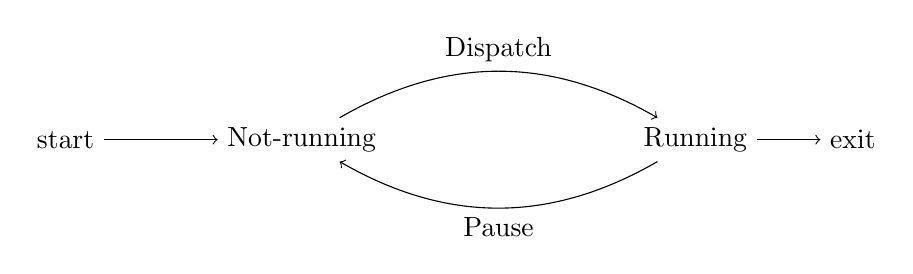
\begin{tikzpicture}
  \node (S) {start};
  \node (NR) [right of=S, node distance=3cm] {Not-running};
  \node (R) [right of=NR, node distance=5cm]  {Running};
  \node (E) [right of=R, node distance=2cm] {exit};
  \path[->] (S) edge node {} (NR)
            (NR)  edge [bend left, above] node {Dispatch} (R)
            (R) edge [bend left, below]  node {Pause} (NR)
            (R) edge node {} (E);
\end{tikzpicture}
\end{center}

In generale, con un solo processore, un solo processo \`e in esecuzione in un certo momento. Lo stato del processo viene scritto nel PCB.

I processi non in esecuzione vengono tenuti in una coda.

\subsubsection{Processo a cinque stati}

% copiare sta roba

\section{I/O devices}

Fra la velocit\`a di input di una tastiera e quella di un cavo Gigabit Ethernet ci sono sette ordini di grandezza. Un processore deve saper gestire input in questo span di velocit\`a.

La prima tecnica introdotta di gestione dei dispositivi I/O \`e quella delle interruzioni. La gestione dei dati attraverso interruzione si distingue fra quella che passa attraverso il processore, e quella che va direttamente alla memoria (DMA - direct memory access).

Interruzione vuol dire che il dispositivo di I/O \`e in grado di mandare un segnale al processore, che salta all'istruzione necessaria per gestire i dati in arrivo.

\subsection{Interruzioni}

Le interruzioni interrompono la sequenza ordinaria delle istruzioni. Servono soprattutto per la gestione dei dispositivi lenti.

Tipologie di interruzioni:
\begin{itemize}
  \item Programmi in esecuzione. Vengono generate dall'ALU, ad esempio per una divisione per 0.
  \item Timer. Vedere multiprocessi.
  \item I/O
  \item Hardware failure, come memory parity error.
\end{itemize}

A volte un'interruzione comporta un cambio di contesto. Altre volte, il programma in esecuzione va in ``ready'' con la priorit\`a che ha.

L'interrupt handler \`e una routine del kernel, fa parte del driver di dispositivo.

Il processore, a seconda di chi gli manda l'interruzione, sa a quale indirizzo deve andare nella RAM per trovare la routine specifica per il dispositivo.

Le istruzioni possono essere mascherate, se sto eseguendo un'istruzione o un blocco di istruzioni importanti, come se sto manipolando strutture dati critiche per il sistema operativo. Ad esempio, se sto manipolando i PCBs. Mascherare le interruzioni \`e importante nella gestione della concorrenza dei processi.

Il controllo per eventuali interruzioni avviene alla fine di ogni istruzione (se le interruzioni non sono state mascherate).

L'idea del fondamentale del DMA \`e che i blocchi di dati sono spostati in memoria senza l'intervento del processore. Il processore viene coinvolto solo all'inizio e alla fine dell'operazione di I/O. All'inizio deve programmare il DMA, dicendogli quali dati deve trasferire e dove. Alla fine riceve l'interruzione.

Una system call \`e un'interfaccia fra il sistema operativo e l'applicazione in esecuzione.

La DMA ha una Control Logic interna, un registro degli indirizzi dove scrivere dove leggere dalla RAM, un ``data register'' dove passano i dati fra RAM e disco. Il ``data count'' dice al DMA quanti bit deve trasferire. La Control Logic accetta comandi ``read'' e ``write'', \`e in grado di segnalare interruzioni, e hanno poi due ``linee'' per il protocollo di interazione con il processore.

Le prime architetture avevano il DMA separato, addetto a tutti i dispositivi I/O, quasi un coprocessore. Attualmente il DMA \`e integrato in ciascun dispositivo di I/O. L'ottimizzazione dello storage \`e partita dalla differenza fra questi due tipi di DMA.

Nel primo caso il DMA separato sovraccarica il System Bus, dovendo trasferire i dati prima dal dispositivo al suo data register, poi dal data register alla memoria.

Un'altra versione ha i dispositivi di I/O su un bus separato (I/O bus) collegato al DMA, che porta poi i dati in memoria.

I file per il sistema operativo sono una sequenza di blocchi di byte, non singoli byte.

I/O Buffering:
\begin{itemize}
  \item Block-oriented
  \begin{itemize}
    \item Information is stored in fixed sized blocks
    \item Transfers are made a block at a time
    \item Used for disks and tapes
  \end{itemize}
  \item Stream-oriented
  \begin{itemize}
    \item Transfer information as a stream of bytes
    \item Used for terminals, printers, communication ports, mouse and other pointing devices, and most other devices that are not secondary storage
  \end{itemize}
\end{itemize}

Un buffer \`e una zona della RAM dove vengono messi i blocchi che arrivano dal disco. Viene gestita come una cache. Velocizza l'I/O in caso di lettura sequenziale. Il DMA scrive sempre nel buffer, perch\'e lo pu\`o trovare sempre essendo il buffer riservato dal sistema operativo.

Dopo che il DMA ha copiato i dati nel buffer, il sistema operativo prende i dati da l\`i e li passa al processo in esecuzione.

Il buffer \`e un punto fisso di riferimento per i dati in transito dai dispositivi di archiviazione alla ram. Senza buffering, il processo deve aspettare che l'operazione si completi.

Il doppio buffering funzioma meglio del buffer singolo. Un buffer viene utilizzato per la lettura dal processo attivo, l'altro viene utilizzato dal DMA per trasferire i dati. Al termine del trasferimento da parte del DMA, il sistema operativo scambia i due buffer.

Buffer circolari: sono un'estensione del buffer doppio. Perch\'e usarne due quando puoi usarne $n$? Si cerca di simulare un buffer ``infinito'', usando $n$ locazioni fisse. Il dispositivo scrive i dati su una delle locazioni. Appena la locazione si riempie, l'utente inizia a leggere da quella locazione e il dispositivo passa alla successiva. Al raggiungimento dell'$n$esima, si riparte dalla prima.

L'insieme delle circonferenze individuate dalla testina in un dato momento \`e detto ``cilindro''.

L'access time di un disco \`e il seek time e il rotational delay. Il resto \`e transfer time.

Se la varianza di velocit\`a del dispositivo e del processo rispetto alla media in un buffer circolare \`e minore della dimensione del buffer circolare, il buffer circolare \`e utile.

\subsection{Scheduling su uniprocessori}

L'ordine in cui si assegnano i processi ad un processore ha impatto sulle prestazioni.

Throughput = numero di processi completati nell'unit\`a di tempo.

Il problema del calcolo delle prestazioni di un processore appartiene alla famiglia dei problemi intrattabili (in generale). Non c'\`e un algoritmo che giri in tempo polinomiale e che trovi una soluzione ottimale al problema dell'ottimizzazione delle prestazioni.

Medium Term Scheduling = mettere su disco processi con bassa priorit\`a per liberare spazio nella ram, necessario a processi pi\`u urgenti.

Un processo sospeso vuol dire che \`e stato messo su disco.

Short term scheduling = dispatcher.
















